\chapter{Introduction}\label{gen:sec:intro}
\markboth{Introduction}{Introduction}
\newcommand{\introOverviewFigure}{
\begin{figure}[h]
    \centering
    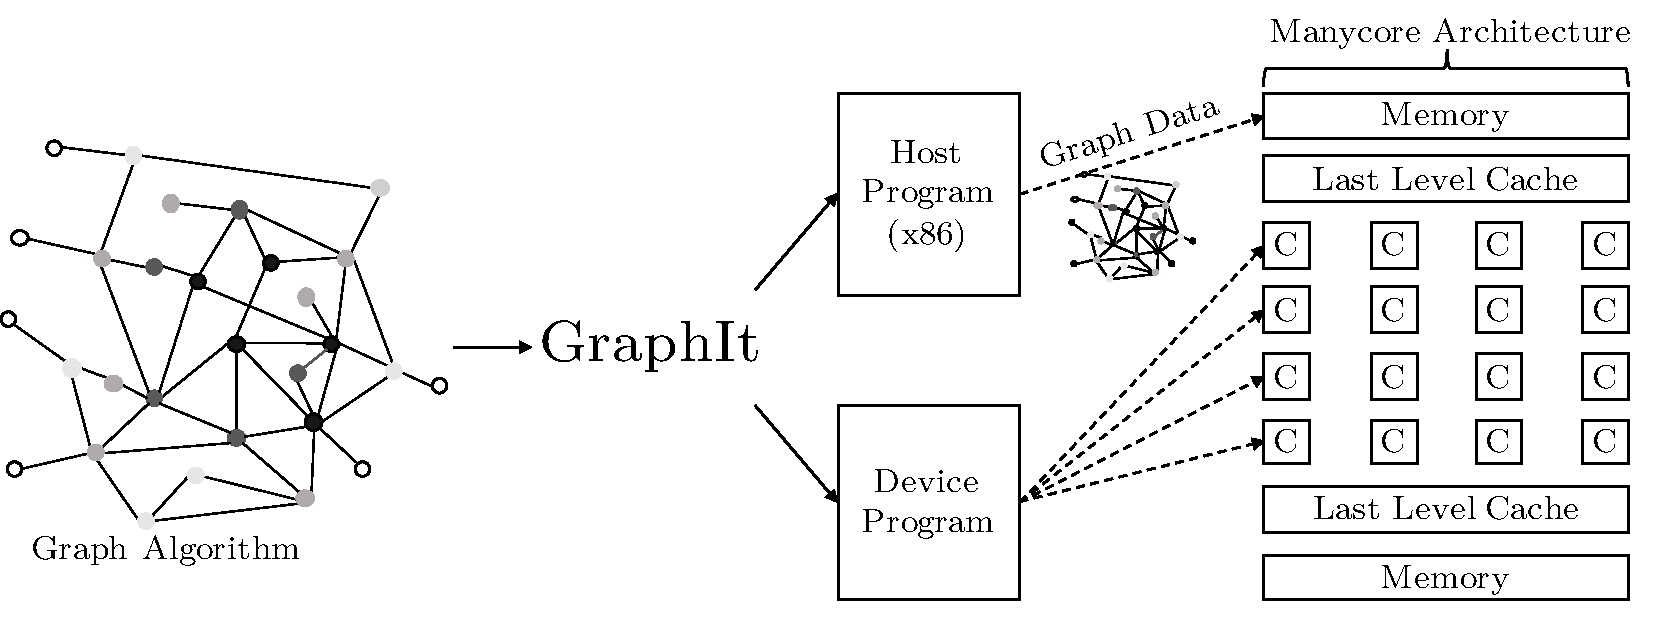
\includegraphics[scale=0.5]{graphit-figures/overview.pdf}
    \caption{This figure shows the flow from Graph Algorithm (e.g. PageRank) to \graphit code to execution on the manycore architecture. 
    Code is generated for both the host and the device. The graph data structure is loaded into device memory by the host program, and the device program is executed in parallel on the manycore architecture.}
    \label{pap:generals:sec:intro:fig:overview}
\end{figure}
}

%\todo{at least one more paragraph here describing graph processing and its importance}

Sparse graph data structures that capture relationships between elements are ubiquitous.
In recent years, the size of graph datasets have exploded~\cite{sahu2017ubiquity} with data coming from fields like networking~\cite{lehmberg2014structure}, social networks~\cite{sharma2016graphjet, eksombatchai2018pixie,kwak2010twitter}, public health~\cite{keeling2005networks, Ulyantsev2016Metafast}, science \cite{tsubaki2019compound,pereira2004detection}, and finance~\cite{boginski2005finance}. 
As graph sizes have grown, so too have the processing requirements. Recommender systems must respond in sub-second latencies \cite{sharma2016graphjet, eksombatchai2018pixie}, and financial algorithms trade on the order of microseconds \cite{menkveld2018hft}.
These challenges have increased the demand for high-performance graph processing systems.

However, implementing high-performance graph processing systems is not as straightforward as simply increasing the number of compute cores or adding more memory bandwidth. 
Further, optimizations used in serial applications or implementations with limited parallelism often do not continue to provide performance when parallelism is increased~\cite{beamer2015locality}.
This has resulted in a wide design space for algorithmic and architectural optimizations to increase the performance of these parallel graph processing systems at scale.


\section{Challenges for Parallel Graph Processing}

Graph processing is notoriously difficult to optimize. 
Performance depends on optimizing locality within sparse data structures, random-access performance, minimizing high-cost communication, and load balancing between parallel threads~\cite{lumsdaine2007challenges, beamer2015locality,satish2014navigating}. 
Worse, the structure of graphs varies widely, both between graphs and between iterations within graph algorithms~\citep{lumsdaine2007challenges, beamer-bfs-direction}. Heuristic optimizations do not benefit all inputs datasets. 
Therefore, graph frameworks must be descriptive enough, and processing hardware must be flexible enough to support them.

These challenges have led to the development of many parallel graph processing frameworks: \graphit~\cite{zhang2018graphit,brahmakshatriya2021compiling,zhang2019optimizing}, GraphLab~\cite{low2010graphlab, low2012distributed}, Grappa~\cite{nelson2015grappa}, GraphChi~\cite{aapo2012graphchi}, Green-Marl~\cite{hong2012green}, and Pregel~\cite{malewicz2010pregel}. 
These frameworks take a user application description and emit parallel code for general-purpose hardware.
Traditionally graph frameworks have targeted CPU and GPU architectures, but newer frameworks also target cloud-resident FPGAs \cite{engelhardt2016gravf, dai2016fpgp}.
These frameworks allow users to focus on exploring optimizations by abstracting the hardware and parallel infrastructure.

Graph processing frameworks are limited by the flexibility and parallelism provided by the hardware they currently target.
Server-class CPUs are widespread and support flexible execution models, but they have limited memory and compute parallelism and poor random-access bandwidth~\citep{beamer2015locality}.
GPUs are also widespread and expose memory parallelism through banking and multiple memory channels, but are limited by vector-like execution models \cite{xu2014graph, shi2018graph}, and have poor random-access bandwidth~\citep{aamodt2018general}.
FPGAs are inherently more flexible than either architecture, but are difficult to optimize when a single recompilation can take hours. 
  
% Solution       
Manycore architectures are composed of hundreds to thousands of efficient general-purpose cores to form a flexible parallel compute fabric.
Past manycore architectures~\cite{ramey2011tilera, agathos2015parallela, gwennap2011adapteva} have been limited by available memory bandwidth and parallelism~\citep{loi2010efficient}.  We employ a manycore design connected to High Bandwidth Memory (HBM) \cite{jedec2020hbm, jouppi2017datacenter} to overcome this issue.
In my thesis, I will show how this manycore architecture can be leveraged to provide high performance on a variety of graph processing applications.


\section{Thesis Overview}
This thesis presents a code generator for graph programs targeting a representative manycore architecture, the \hbmc. 
Within this code generator, I implement and evaluate manycore specific optimizations to improve graph processing performance. 
While graph processing frameworks and optimizations on parallel systems is an active area of research, this work targets a novel manycore architecture.
Further, the optimizations for this architecture expand the space and provide a new class of techniques for graph applications on this emerging architecture. 

In this thesis, I focus on two different aspects of the problem of efficiently utilizing the \hbmc for graph processing: ease of programming and manycore-specific optimizations. 
Reasoning about the implementation of a graph application and the details of the underlying architecture can be difficult especially as techniques for obtaining performance on architectures become increasingly complex. 
I address this by building a code generator that allows the user to reason about the graph application and optimizations at a high level without requiring knowledge of the underlying manycore architecture.
I use observations about the \hb architecture to implement existing graph processing optimizations and introduce several manycore specific optimizations that build off of the observation that most graph applications are memory bound. 
%I propose further study of performance on the manycore in order to optimize a variety of techniques and applications (\ref{gen:sec:proposed}).


%I use information gained through experimentation with the manycore architecture to optimize graph applications (\ref{sec:method}) and build these optimizations into a code generation engine (\ref{sec:method:sub:baseline}).
\section{Organization}
%\todo{give a roadmap of each chapter and its contributions/contents}

I begin this thesis by providing background information on graph processing and introduce the algorithms and graphs that are used for evaluation.
I also give an overview of the \graphit DSL and the \hbmc architecture that I target in Chapter~\ref{gen:sec:background}.

In Chapter~\ref{gen:sec:optimizations}, I present the set of optimizations that we implement and explore in this thesis.
This includes several existing graph processing optimizations as well as the \hbmc-specific optimizations introduced in this thesis.
These optimizations target things such as load balancing, graph traversal, and the \hb memory system. 

I then introduce the code generation framework that I implemented as a backend to the \graphit DSL in Chapter~\ref{gen:sec:graphitbackend}.
This chapter describes how optimizations are applied to programs and what the resulting generated manycore code includes.

Next, Chapter~\ref{sec:eval} presents an evaluation of the code generation framework and the set of optimizations introduced in Chapters~\ref{gen:sec:optimizations} and~\ref{gen:sec:graphitbackend}.
We evaluate the performance of each optimization on a variety of input graphs and algorithms.
%
Before concluding, I contextualize my work within the space of graph processing frameworks and optimizations in Chapter~\ref{gen:sec:relatedwork}.
I then conclude and provide some insights into areas of future work in Chapter~\ref{gen:sec:conclusion}.
%Then, I provide background information on the \graphit DSL and the representative manycore architecture that I target in Section~\ref{gen:sec:background}.
%In Section~\ref{gen:sec:graphitbackend}, I present my work implementing a code generation backend for the \graphit DSL. 
%I further propose manycore specific optimizations in Section~\ref{gen:sec:graphitbackend} and discuss the implementation of several other graph processing optimizations. 
%Finally, Section~\ref{gen:sec:proposed} presents two areas of work that I plan to pursue in the completion of my thesis: a study and analysis of tunable parameters to find optimal values for various graph optimizations and a manycore implementation of multi-source BFS.


% In this paper, we outline a general execution model for this class of manycore systems.
% We then describe a prototypical computational model for graph processing applications that provides computation and memory parallelism.
% %Manycore architectures introduce a level of complexity that can make it difficult to reason about how best to obtain performance in graph application code.
% It can be challenging to write code for manycore architectures that exploits the
% right types of parallelism to maximize performance for an application.

